\documentclass{article}
\usepackage[english]{babel}
\usepackage{amsmath}
\usepackage{graphicx}
\usepackage{hyperref}

\title{Milner's scheduler}
\author{Adrián Enríquez Ballester}

\begin{document}
\maketitle

We want to specify a simple scheduler for a set of $n$ agents 
$P_1,..., P_n$. Each agent $P_i$ performs a task repeatedly, 
and the scheduler is required to ensure that they begin the 
task in cyclic order starting with $P_1$. The different 
task-performances need not exclude each other in time. 
For example, $P_2$ can begin before $P_1$ finishes, but the 
scheduler is required to ensure that each agent finishes 
one performance before it begins another.

We assume that $P_i$ requests task initiation by an action 
$a_i$ and signals completion by an action $b_i$. The 
scheduler can then be specified by requiring that:

\begin{itemize}
  \item It must perform $a_1,...,a_n$ cyclically, starting 
    with $a_1$.
  \item It must perform $a_i$ and $b_i$ alternately for each $i$.
\end{itemize}

However, a scheduler which imposes a fixed sequence, say 
$a_1b_1a_2b_2...$ is not good enough, 
the scheduler must allow any sequence of actions compatible with 
the two conditions above. For example, for $n=2$, the sequences 
$a_1a_2b_1b_2a_1$ and $a_1b_1a_2a_1b_2b_1$ are compatible with 
the specification, but the sequences $a_1b_1a_1$ and 
$a_1b_1a_2a_1a_2$ are not.

\section{Petri net model for two processes}

The Figure \ref{fig:diagram} shows a diagram of the Petri net 
for the Milner's scheduler where $n=2$. Each process has two 
places which represent its two possible states (i.e. idle or 
working), and two transitions $a_i$ and $b_i$ for the 
corresponding actions of starting and ending its task.

The scheduler state has been modeled with one place per process,
which reflect the one that has to start next. The token 
changes from a place to the next one when the corresponding 
$a_i$ transition is fired, allowing only the one which corresponds
to the current state.

\begin{figure}
  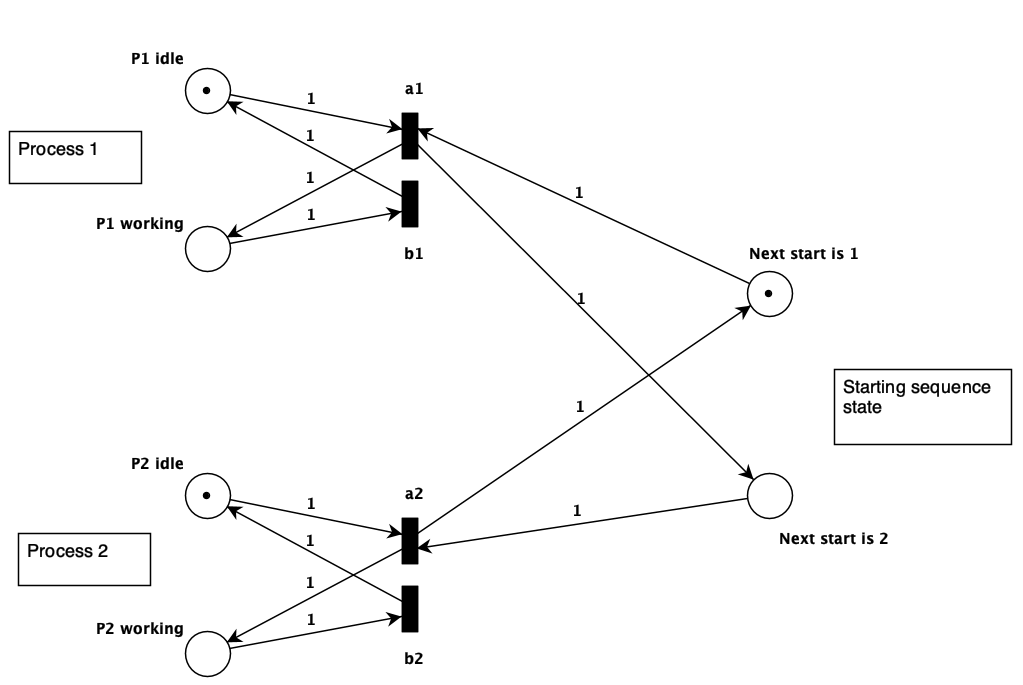
\includegraphics[width=\textwidth]{milner-scheduler-net.png}
  \caption{
    Petri net diagram for the Milner's scheduler 
    of two processes
  }
  \label{fig:diagram}
\end{figure}

\section{Properties}

If we traverse the reachability graph of the net at the 
Figure \ref{fig:diagram}, we reach $8$ different markings. 
Every transition appears in the graph and we can reach again 
the initial marking from any other, so the net is live.

Also, as intended for properly modeling the states, every place 
is $1$-bounded, thus the net itself is $1$-bounded.

\section{Generalization}

The Petri net model can scale to $n$ processes in the following way:

\begin{itemize}
  \item For each $i \in \{1,...,n\}$, a process is represented with 
    two places for its idle and working state, and two transitions 
    $a_i$ and $b_i$ connected as in the example for $n=2$. For the 
    initial marking we can put a token in its idle place.
  \item For each $i \in \{1,...,n\}$, a place $p_i$ for the scheduler 
    sequence state. $p_i$ should be a precondition of $a_i$ and a 
    postcondition of $a_{i-1}$ ($a_{n}$ when $i$ is $1$). For the 
    initial marking we can put a token in $a_1$.
\end{itemize}

\section{Reachable markings growth}

Each process can be either idle or working, and for each state of the 
scheduler sequence it is possible to reach any combination of the 
process states. For a Milner's scheduler of $n$ agents, as there are 
$n$ agents with $2$ states each one, and the scheduler sequence has $n$ 
states, the amount of reachable markings of its Petri net $(N, M_0)$ is 
as follows:

$$\big|[M_0\rangle\big| = 2^n \cdot n$$

\end{document}
